% 正文的中文、符号采用宋体小四,阿拉伯数字及西文字母、符号采用Times New Roman,小四。
\documentclass[UTF8,zihao=-4]{ctexart}
\setCJKmainfont[BoldFont=SimHei]{SimSun}
\setCJKsansfont{SimHei}
\setmainfont{Times New Roman}
\setmonofont{Consolas}
\usepackage{geometry}
\usepackage{setspace}
\usepackage{graphicx}
\usepackage{fancyhdr}
\usepackage{pdfpages}
\usepackage{float}
\usepackage[font=small]{caption}
\usepackage{listings}
\usepackage{pythonhighlight}
\usepackage{pgfplots}               % 使用pgfplots绘图工具包
\usepackage{amsmath}
 \usepackage{textcomp}
 \usepackage{booktabs} % 三线表
\pgfplotsset{width=12cm,compat=1.13} % 图片绘制的宽度是7cm,使用的pgfplots版本为1.13
\pagestyle{fancy}
% 设计(论文)除封皮外,各页均应加页眉,单线上居中打印页眉文字,页眉文字均为宋体五号“长春理工大学本科毕业设计”或“长春理工大学本科毕业论文”。
\chead{\songti\zihao{5}长春理工大学本科毕业设计}
\lhead{}
\rhead{}
% 设计(论文)页码:宋体,小五,页面底端居中
\cfoot{\songti\zihao{-5}\thepage}
\geometry{a4paper,left=3.17cm,right=3.17cm,top=2.54cm,bottom=2.54cm}  %上下边距2.54cm,左(+装订线0cm)右边距3.17cm,
\title{基于朴素贝叶斯的垃圾邮件过滤算法}
\author{150521310 何程斌}
\date{}
\renewcommand{\abstractname}{}
\renewcommand{\theequation}{\arabic{section}-\arabic{equation}}
\renewcommand{\thetable}{\arabic{section}-\arabic{table}}
\renewcommand{\thefigure}{\arabic{section}-\arabic{figure}}
\renewcommand\labelenumi{(\theenumi)}
\newcommand{\upcite}[1]{\textsuperscript{\cite{#1}}}
\ctexset{
  % 各章一级标题序号及标题:宋体三号加粗居中
  % 目录标题貌似也是 section 标题格式控制
  % 目录题头为三号宋体字加粗居中书写,目录中各章题序及标题均用宋体,小四;多倍行距1.25,页码对齐,目录自动生成。
  section = {
    name = {第,章},
    format+=\songti\zihao{3}\textbf\centering
  },
  % 各章二级标题序号及标题:宋体四号加粗,缩进2个字符;
  subsection = {
    format+=\songti\zihao{4}\textbf
    % indent=2\ccwd
  },
  % 各章三级标题序号及标题(含三级标题以下标题):宋体小四加粗,缩进2个字符。
  subsubsection = {
    format+=\songti\zihao{-4}\textbf
    % indent=2\ccwd
  }
}
\begin{document}
% 封面页
\includepdf[page=1-2]{论文封面.pdf}

% 摘要、目录等正文之前的页码用罗马数字(I、II、III……),且分别编码
% 设计(论文)的中文和外文摘要置于目录前,并编入目录。
\pagenumbering{Roman}
\section*{摘要}
  \addcontentsline{toc}{section}{摘要}
  % 中文摘要题头选用模板中样式所定义的“标题1”,居中;宋体,居中,三号,加粗;多倍行距1.25,段前0行,段后1行,取消网格对齐。
  %\addvspace{0.5\baselineskip}

  % 摘要正文选用模板中样式所定义的“正文”,段落首行缩进2个字符,宋体,小四;多倍行距1.25,段前、段后均为0行,取消网格对齐。
  \linespread{1.25}\songti\zihao{-4}
   近些年随着互联网的快速发展,电子邮件得到了十分充足的应用,但伴随而来的是日益严峻的垃圾邮件问题。本文首先介绍了垃圾邮件过滤的课题背景和国内外研究现状,然后介绍了朴素贝叶斯算法,接着提出了一种基于朴素贝叶斯算法的垃圾邮件过滤算法,使用伯努利模型计算方法对过滤算法进行了流程设计与代码实现。在trec06数据集上运行了测试,采用交叉验证方法计算出算法性能评估指标,分析了训练集大小、禁用词表对过滤算法性能的影响,最后证明该垃圾邮件过滤算法的有效性。
   \\
   

  % 关键词与摘要之间空一行。中文关键词之间用2个空格间隔,黑体小四顶格书写。
  {\noindent\heiti\zihao{-4}\textbf{关键字:}朴素贝叶斯;反垃圾邮件;邮件分类}
  % \end{spacing}
\newpage

\section*{Abstract}
  \addcontentsline{toc}{section}{Abstract}
  % 外文摘要题头“Abstract”不可省略。标题“Abstract”选用模板中的样式所定义的“标题1”,居中;Times New Roman,居中,三号,加粗;多倍行距1.25,段前0行,段后1行,取消网格对齐。
  % \addvspace{0.5\baselineskip}

  % Abstract正文设置:段落首行缩进2字;Times New Roman,小四;多倍行距1.25,段前、段后均为0行,取消网格对齐。
  \linespread{1.25}\zihao{-4}
	In recent years, with the rapid development of the Internet, e-mail has been widely used, but the problem of spam has become increasingly serious. Firstly, the background of spam filtering and the research status are introduced. Then, the naive Bayes algorithm is introduced. Then a spam filtering algorithm based on naive Bayes algorithm is proposed, which is filtered by Bernoulli model. Then the process design and the code implementation are introduced. The test was run on the trec06 dataset. The cross-validation method was used to calculate the performance evaluation index. The effect brought by size of the training set and the stop-words on the performance of the filtering algorithm were analyzed. Finally, the effectiveness of the spam filtering algorithm was proved.
	\\

  % Key words与Abstract正文之间空一行。Key words之间用分号间隔,Times New Roman,小四,顶格书写。
  \noindent\zihao{-4}\textbf{Key Words: }Naive Bayes, Anti-Spam, E-mail Classification
  % \end{spacing}
\newpage

% TOC 页
\linespread{1.25}
\tableofcontents
\newpage

\songti\zihao{-4}
% 正文以后的页码用阿拉伯数字(1、2、3……)编排页码
\pagenumbering{arabic}
\newpage
\section{绪论}
\subsection{本课题研究的目的及意义}
随着互联网的飞速发展,电子邮件越来越普及,逐渐成为人们生活与工作中不可缺少的交流工具。但是,在带来便利的同时,电子邮件也给人们带来了不少令人无法忽视的问题,其中最严重的问题莫过于数量不断增长的垃圾邮件。据Securelist(卡巴斯基实验室旗下的IT安全信息资源网站)于2017年公布的全球垃圾邮件报告显示,2017年第三季度,全球的电子邮件中有58.02\%是垃圾邮件;9月份垃圾邮件占比最高,为59.56\%;中国是垃圾邮件的最大发信国,为12.24\%,越南排在第二位(11.17\%),美国排在第三位(9.62\%),印度位居第四(8.49\%)\cite{securelist}。垃圾邮件占据了网络中巨大的带宽资资源,对用户的日常工作生活带来了极大的困扰。并且,不少垃圾邮件还附带着病毒软件和诈骗链接,给用户的计算机、甚至个人财产带来了威胁。

朴素贝叶斯分类器是在特征之间相关性较弱的条件下基于贝叶斯定理的分类算法,是文本分类领域的一种热门算法,并且在垃圾邮件识别领域中已有了非常成熟的应用。

本文基于朴素贝叶斯算法实现了一个简单垃圾邮件过滤算法。以大量合法邮件和垃圾邮件作为样本,提取正文,建立特征词库。然后进行有督导的学习,实现了对垃圾邮件进行高准确率的识别分类。

\subsection{国内外研究现状}

将英文文本转换为单词集合非常简单且精确,因为在英语单词之间存在自然分割符号。相比之下中文比英语要复杂的多,一句话可能包含很多含义,它没有独立有效的语义,在不同语境下同一句话甚至能够体现了不同的语义。因此,与国内垃圾邮件分类的发展相比,国外发展快得多。

总体来讲,目前主要有以下几种垃圾邮件过滤技术。
\begin{enumerate}
	\item 黑白名单过滤\upcite{anti-spam}:把频繁制造并发送垃圾邮件的域名/IP 加入黑名单中。当收到新邮件时查询发件人的域名或者IP是否在黑名单中,并拒收这些黑名单发件人的邮件\cite{zhangpei}。白名单中的发件人则代表得到用户信任的发件人,他们发送的邮件会直接被视为合法邮件,不经过更进一步的检查。但如果对方采用代理IP、伪造地址等手段发送邮件时,该方法就失效了。并且,该方法也十分依赖用户手动标记黑白名单发件人,用户花费的时间成本较大。
	\item 关键词过滤:创建垃圾邮件的特征关键词表,当收到新邮件时判断此邮件正文中是否存在这些非法关键词。但该方法太过粗放,带有非法关键词的正常邮件也会被视为垃圾邮件拦截,并且为达到足够的垃圾邮件过滤度这种技术需要建立一个庞大的特征关键词表。为了绕过关键词检测,垃圾邮件的发件人也可以在关键词中间插入分隔符号,例如将“开发票请联系某某某”转为“开 \textyen 发 \textyen 票 \textyen 请 \textyen 联 \textyen 系 \textyen 某 \textyen 某 \textyen 某”的形式。
	\item 规则评分过滤:通过对大量邮件的综合分析, 得到一个庞大的规则库。规则库里的每条规则都对应一个分数,计算收到的新邮件获得的分数\cite{zhangpei},总分超过特定的阈值时该邮件就会被判定为垃圾邮件。但因规则数量有限,无法检测匹配规则条数为0的邮件。决策树是规则评分过滤技术的代表,最早出现的决策树相关的学习系统是Hunt于1966年研发的;1979 年,Quinlan 提出了迭代分类器 ID3 算法;1983年他又提出了 C4.5 算法\upcite{haibo,wux},改进了ID3 算法不能处理连续值属性数据的缺点;该算法随着数据的不断增加而加以调整,弥补了 ID3 算法的不足之处\cite{caocuiling}。这些算法虽然在一定程度上能够 满足需求,但是它们的根本原理都是预设规则比较结果来判定是否为垃圾邮件。同时这些规则 往往都是静态的,缺少自助学习策 略,在规律不明显的应用领域中过滤效果很差。
	
	\item 内容过滤:它可以分为规则角度和内容统计。本文研究的垃圾邮件过滤算法基于朴素贝叶斯算法,是内容统计的算法。该算法速度快、效率高、耗时短、准确性高,同时还具有自我学习功能,能够不断地动态调整垃圾邮件集和合法邮件集的概率。在文本分类领域具有十分广泛的应用。垃圾邮件过滤领域中最常用的算法便是朴素贝叶斯算法和支持向量机算法\upcite{yanglei}。马小龙提出了 SVM-EM 朴素贝叶斯算法,该算法先利用SVM 算法将数据集分成完整集和缺失集,计算缺失属性数据项与完整属性数据项的相关度,利用EM 算法对数据不完整属性进行修补处理,最后利用朴素贝叶斯算法分类\cite{maxiaolong}。
\end{enumerate}

\subsection{本文的组织结构}
	本文共五章,文章结构如下:
	
	第一章绪论。描述了朴素贝叶斯算法和垃圾邮件过滤的研究内容,国内外研究现状。并提出了本文的主要研究内容。
	
	第二章朴素贝叶斯算法。介绍了朴素贝叶斯算法的基本概念、详细计算步骤和三种朴素贝叶斯模型,为之后的章节奠定坚实的理论基础。
	
	第三章垃圾邮件过滤算法实现。首先介绍了垃圾邮件的特征等基本概念,结合第二章介绍的朴素贝叶斯算法,详细描述了将朴素贝叶斯算法应用于垃圾邮件过滤领域的过程。
	
	第四章算法改进。介绍了第三章的算法实现的不足,分析了问题出现的原因,以及提出了改进算法的方法。
	
	第五章系统测试与评估。本章是本文的重点,对算法进行对比测试,得到了准确率、精确率、召回率等评估数据,并分析了训练集大小、禁用词表对实验结果的影响,由此验证了本文提出的算法的可行性和有效性。

\newpage
\section{朴素贝叶斯算法}
\subsection{朴素贝叶斯算法分析}
	贝叶斯定理的核心思想为统计各个特征的概率数据来计算未分类的样本被分类为各个类别的概率,比较概率选择概率最大的那个分类作为最终分类。贝叶斯定理由条件概率公式和全概率公式推导而来。
	
	条件概率指在事件$B$发生的前提下,事件$A$发生的概率\cite{bayes},对应的公式即为$P(A|B)=\frac{P(A\cap B)}{P(B)}$,将右侧的分母移到左侧后可以得到:
	\begin{equation}
	\label{equ:cond-prob-pab}
	P(A \cap B)=P(A|B) \cdot P(B)
	\end{equation}

	
	同理可得:
	\begin{equation}
	\label{equ:cond-prob-pba}
	P(A \cap B) = P(B|A) \cdot P(A)
	\end{equation}

	
	结合公式\ref{equ:cond-prob-pab}和公式\ref{equ:cond-prob-pba}我们可以发现,$P(A|B) \cdot P(B)=P(B|A|) \cdot P(A)$,由此就得到了条件概率的计算公式:
	
	\begin{equation}
	\label{equ:cond-prob}
	P(A|B)=\frac{P(B|A) \cdot P(A)}{P(B)}
	\end{equation}
	
	全概率公式\upcite{bayes}假设$S$为样本空间,$\langle A_1,A_2,\cdots,A_n \rangle$是$S$的一个划分(即$S=\sum\limits_{i=1}^{n}A_i \text{,} P(A_i)>0$)。$B$ 为$S$的某一事件,在这种情况下,事件$B$可以被分为$n$个部分,即$P(B)=\sum\limits_{i=1}^{n}P(B\cap A_i)$,在先前的推导中我们已知$P(B \cap A)=P(B|A) \cdot P(A)$,相互结合就可得到全概率公式:
	\begin{equation}
	\label{equ:full-prob}
	P(B)=\sum\limits_{i=1}^{n}P(B|A_i) \cdot P(A_i)
	\end{equation}

	
	将全概率公式代入条件概率公式,就得到了贝叶斯公式:
	\begin{equation}
	\label{equ:bayes}
	P(A|B) = \frac{P(B|A) \cdot P(B)}{\sum\limits_{i=1}^{n}P(B|A_i) \cdot P(A_i)}
	\end{equation}
	
	用一个$n$维特征向量$\vec{f}$来表示待分类的样本$d$,其中$f_i(i=1,2,...,n)$表示第$i$个特征,$n$是特征的个数。则该样本$d$分类为$c_j(j=1,2,...,m)$的概率为:
	
	\begin{equation}
	\label{equ:nb}
	P(C=c|\vec{F}=\vec{f})=\frac{P(\vec{F}=\vec{f}|C=c)\cdot P(C=c) } {P(\vec{F}=\vec{f})}
	\end{equation}
	
	其中,$P(\vec{F}=\vec{f})=\sum\limits_{j=1}^{m} P(C=c_j) \cdot P(\vec{F}=\vec{f}|C=c_j)$
	
	但是,$P(\vec{F}=\vec{f}|C=c)$往往很难计算($\vec{F}$可能有许多不同的值,并且也存在数据稀疏的问题),这导致贝叶斯定理的直接使用是十分困难的。
	
	而朴素贝叶斯算法则基于贝叶斯定理,进一步做出了所有特征都相互独立的假设。与贝叶斯定理相比较,对于特征向量为$\vec{f}=\langle f_1, \ldots, f_n \rangle$的待分类样本$d$,其被分类为$c$分类的概率为:
	
	\begin{equation}
	P(C=c|\vec{F}=\vec{f})=\frac{P(C=c) \cdot \prod\limits_{i=1}^{n} P(F_i=f_i|C=c)} {P(\vec{F}=\vec{f})}
	\end{equation}
		
	同时,$P(\vec{F}=\vec{f})=\sum\limits_{j=1}^{m} P(C=c_j) \cdot \prod\limits_{i=1}^{n}  P(F_i=f_i|C=c_j)$
	
	由于$P(\vec{F}=\vec{f})$对于任意分类都是相同的,所以可以将公式进一步省略为:
	
	\begin{equation}
	P(C=c) \cdot \prod\limits_{i=1}^{n} P(F_i=f_i|C=c)
	\end{equation}
	
	所以,仅需计算所有分类对应的该公式的值,比较大小,即可完成分类,这极大地降低了计算难度。
	
	朴素贝叶斯算法是最被广泛应用的两种分类算法中的一种,另一种是决策树算法。和决策树算法相比,朴素贝叶斯算法源自古典数学理论,拥有坚实的数学基础,以及稳定的分类效率\cite{nb}。朴素贝叶斯算法需要的计算参数并不多,对数据的完整性也没有苛刻的要求。因此,相比起来,朴素贝叶斯算法的实现更简单。从理论上来说,朴素贝叶斯算法具有最小的误差率。然而实际应用上并非总是如此。因为朴素贝叶斯算法是以特征之间非强关联这一假设为基础,这一假设在实际应用中并不是总是成立的。所以,在这一假设不成立的应用场景中,朴素贝叶斯算法的分类准确率稍为逊色。但研究表明在特定领域(如文本分类)中,朴素贝叶斯算法对分类结果的准确性的影响并不大。

	
\subsection{朴素贝叶斯的三种常用模型}
\subsubsection{高斯模型}
	若特征 $f_i $为连续变量,则可以假设特征分布符合高斯分布(正态分布),即假设每个分类 $c_j$ 下的特征 $f_{ji}$ 符合高斯分布。然后我们就可以通过高斯分布的概率密度函数来计算样本 $d_k$ 中某个特定值的条件概率 $P(F_i=f_i|C=C_j)$ 。高斯分布的概率密度函数为: 
	
	\begin{equation}
	f(d ; \mu, \sigma)=\frac{1}{\sigma \sqrt{2 \pi}} \exp \left(-\frac{(d-\mu)^{2}}{2 \sigma^{2}}\right)
	\end{equation}
	
	其中 $\mu$ 是均值, $\sigma^2$ 是方差。 假设在类别 $C_j$ 中,特征 $f_i$的均值为 $\mu_{ji}$ ,方差为 $\sigma_{ji}^2$(这两项可以通过样本数据统计出来)。则 
	
	\begin{equation}
	P\left(F_i=f_{i} | C=c_{j}\right)=\frac{1}{\sigma_{ji} \sqrt{2 \pi}} \exp \left(-\frac{\left(f_{i}-\mu_{ji}\right)^{2}}{2 \sigma_{ji}^{2}}\right)
	\end{equation}
	
	为了解决数值连续的问题,我们还可以将连续数值离散化。通常当训练样本数量较少时,直接计算概率分布的方法是最合适的。 而在样本数量较多的情况下,将数值离散化的方法相比之下则更加表现优异。在实际应用场景中,我们往往会在海量的数据样本的基础上进行训练,在这种情况下更适合使用离散化方法,而不是计算概率分布的方法。
\subsubsection{多项式模型}
	若特征$f_i$是离散值,可以假设它符合多项式分布。可以统计 $f_i $的某个特征在样本中的频率来估算其概率。 假设 特征$ f_i$ 有 $S_i $个可能的取值,并且在n个样本中,类别为 $c_j$ 、特征 $f_i $取值为 s 的样本有 $m_{jis}$ 个。则
	\begin{equation}
		P(f_{i} | C=c_{j})=m_{j i s} / m_{j}
	\end{equation}
	
	将一短文本转化为长度为该文本词语数量(词语可以重复)的特征向量。特征向量的分量值为该位置的单词在词典中的下标,假设词典长度为 $n$,则分量值的取值范围为$\{1,2,\dots,n\}$。
	
	
\subsubsection{伯努利模型}
    如果特征 $f_i$ 是稀疏二项离散值,可以假设它符合 伯努利分布。伯努利分布只有两种可能的取值,我们将其编码为 {0,1},则

	\begin{equation}
    P(f_i|C=c_j)=\begin{cases}
    		{P(f_i=1|C=c_j)} \\ 
    		{P(f_i=0|C=c_j)=1-P(f_i=1|C=c_j)}
    		\end{cases}
	\end{equation}

    比如构造一个5000个不同单词的向量作为输入特征$\vec{w}$,对于一段文本,其中有出现的单词,在$\vec{w}$中对应单词的位置设为1,其它位置为0,这样$\vec{w}$中的每个特征(单词)的取值为1或0,符合伯努利分布。
\subsubsection{本设计采用的模型}
	本设计使用伯努利模型。用向量$\vec{w}(m \times 1)$表示一个$m$个单词的字典。当邮件中出现字典$\vec{m}$中的第$i$个单词时,将$w_i$置1,否则置0。例如对于一封具$n$个词语的邮件,它的特征向量为:
	
	$$
	\vec{w}=
	=
	\begin{bmatrix}
	w_1\\
	w_2\\
	w_3\\
	\vdots\\
	w_i\\
	\vdots\\
	w_m
	\end{bmatrix}
	=
	\begin{bmatrix}
	1\\
	0\\
	1\\
	\vdots\\
	0\\
	\vdots\\
	1
	\end{bmatrix}
	\begin{matrix}
	\text{今天}\\
	\text{公司}\\
	\text{促销}\\
	\vdots\\
	\text{欢迎}\\
	\vdots\\
	\text{选购}
	\end{matrix}
	$$
	
	邮件包含“今天”、“促销”、“选购”等词,因此字典中的对应位置设为1。字典中未在邮件中出现过的词,则将对应的位置设为0。 而对于邮件中某些词可能并未出现在字典中,我们可以直接忽略这些词。
	

\newpage
\section{垃圾邮件过滤算法实现}
\subsection{系统设计}
	邮件分类的具体实现步骤,如流程图\ref{fig:overall-flowchart}所示:
	
	\begin{figure}[H]
		\centering
		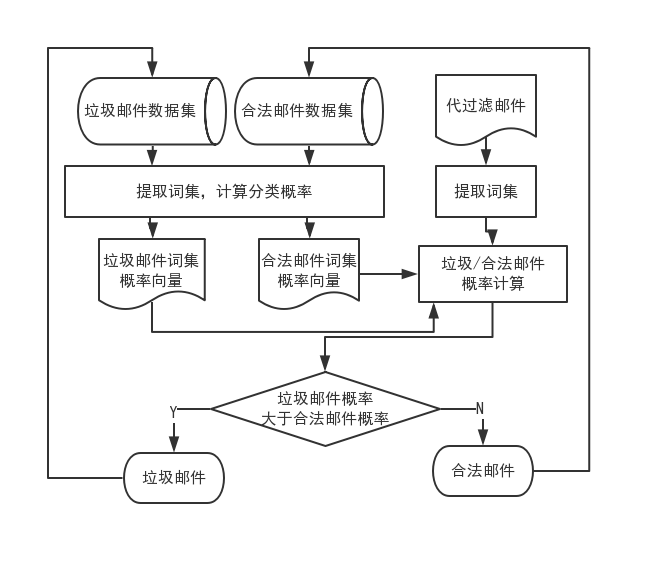
\includegraphics[scale=0.5]{pictures/朴素贝叶斯算法的垃圾邮件过滤算法的流程图.png}
		\caption{基于朴素贝叶斯算法的垃圾邮件过滤算法流程图}
		\label{fig:overall-flowchart}
	\end{figure}

	\begin{enumerate}
		\item 对收集到的大量的垃圾/合法邮件作为训练集进行中文分词。
		\item 将训练集中的每封邮件以词语作为特征转化成对应的特征向量。然后对每个分类(垃圾/合法)依次计算每个特征对于该分类的概率,得到每个分类的分类特征概率向量。
		\item 使用朴素贝叶斯算法,基于分类特征概率向量对待分类邮件进行分类。
	\end{enumerate}

	由此可以发现,整个垃圾邮件过滤系统需要三个方面的问题,一是对大量的邮件数据集进行分词处理,二是对现有的邮件数据集进行计算特征分类概率,三是对待分类的新邮件进行分类过滤。按此思想设计,得到如图\ref{fig:overall-structure}所示的系统架构图。
	
	\begin{figure}[H]
		\centering
		\setlength{\abovecaptionskip}{0.cm}
		\setlength{\belowcaptionskip}{-0.cm}
		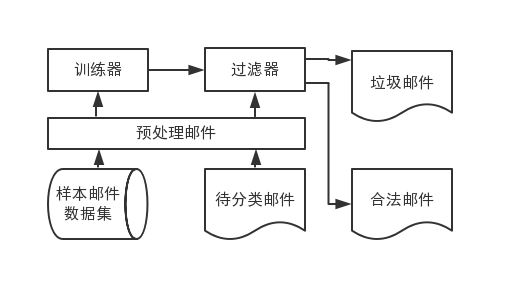
\includegraphics[scale=0.5]{pictures/系统总体架构图.png}
		\caption{系统总体架构图}
		\label{fig:overall-structure}
	\end{figure}

	依照此架构,可以将系统分割成三部分实现:
	
	第一部分用于对邮件进行预处理,如图\ref{fig:preprocess-system}所示。
	当数据集足够大时,分词这一步骤是十分耗时的。对于trec06数据集来说大约有61810封邮件样本,要完成所有61810封邮件样本的分词大约需要27分钟,这给程序的调试运行带来了极大的困难。为解决该问题,本设计将分词这一步骤独立成单独的系统。并保存分词后的结果,留作稍后的训练步骤使用,从而加快系统运行效率。
	\begin{figure}[H]
		\centering
		\setlength{\abovecaptionskip}{0.cm}
		\setlength{\belowcaptionskip}{-0.cm}
		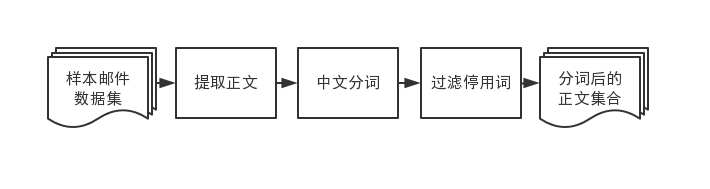
\includegraphics[scale=0.45]{pictures/邮件预处理子系统.png}
		\caption{邮件预处理子系统}
		\label{fig:preprocess-system}
	\end{figure}
	
	第二部分用于对过滤器进行训练,如图\ref{fig:train-system}所示。
	训练子系统在预处理子系统处理后得到的正文词语表集合上进行训练。并且,训练算法这一步骤并非每进行分类一次便要进行一次,我们只需要训练出一个准确率足够高的模型,便可供分类步骤循环使用,所以,训练步骤可以单独成一个子系统。
	\begin{figure}[H]
		\centering
		\setlength{\abovecaptionskip}{0.cm}
		\setlength{\belowcaptionskip}{-0.cm}
		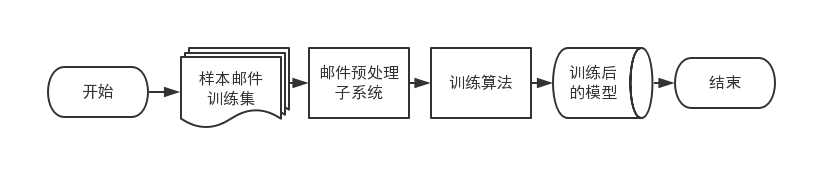
\includegraphics[scale=0.45]{pictures/邮件训练子系统.png}
		\caption{过滤器训练子系统}
		\label{fig:train-system}
	\end{figure}
		
	第三部分用于对待分类邮件进行分类过滤,如图\ref{fig:predict-system}所示。分类子系统使用训练子系统得到的模型对待分类邮件进行分类。还可以将分类子系统设计成如 HTTP API 后端程序等形式作为守护进程运行,供外部程序(如邮件客户端)调用接口。
	\begin{figure}[H]
		\centering
		\setlength{\abovecaptionskip}{0.cm}
		\setlength{\belowcaptionskip}{-0.cm}	
		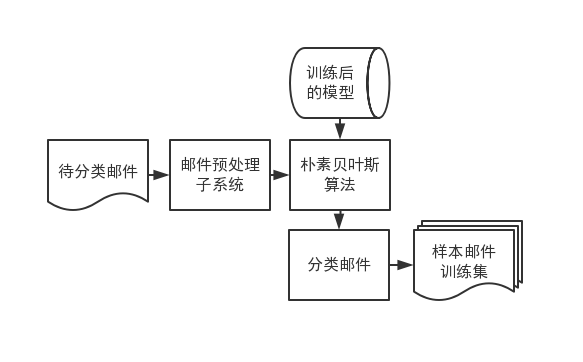
\includegraphics[scale=0.45]{pictures/邮件分类子系统.png}
		\caption{邮件分类子系统}
		\label{fig:predict-system}
	\end{figure}


\subsection{数据集预处理}
	本设计采用公开的垃圾邮件数据集  trec06。trec06 是一个由国际文本检索会议提供的垃圾邮件数据集,共有中文和英文两个子集。trec06数据集收集于现实生活中的真实的邮件,同时还保留了邮件的原始文本格式。本设计仅使用 trec06 的中文数据集部分 trec06c,大约有 61810 条数据。

	根据多用途互联网邮件扩展(MIME)标准,对邮件格式进行解析,提取正文,对内容进行分词、过滤停用词后,依照邮件类别以纯文本文件的格式分类存储。
		
	本设计使用的中文分词工具包为北京大学于 2019 年 2 月开源的 pkuseg\upcite{pkuseg}。与业界其他工具包(如 jieba、snownlp 等)相比,pkuseg 在特定的数据集上拥有更高的分词准确率。根据北大研究组的测试结果, pkuseg 分别在示例数据集(MSRA 和 CTB8)上降低了 79.33\% 和 63.67\% 的分词错误率\cite{pkuseg}。
	
	停用词指在自然语言处理中,为节省存储空间、提高处理效率,会过滤掉某些低价值的字或词,如“这”、“那”、“一个”,这些字或词即被称为停用词(Stop Words)\upcite{stopwords}。这些词往往没有具体语义,在文中仅仅用作助词等。这些词对文本的特征识别并无帮助,反而会增大时空开销。所以,实际应用中往往会预先过滤掉停用词。本设计将哈工大停用词表、百度停用词表和四川大学机器智能实验室停用词库作并集,得到了2313个词语,将其作为本设计的停用词表。
	
	整个trec06数据集有两个文件夹。data文件夹存储原始的邮件文本。data文件夹中有209个子文件夹,而每个子文件夹又各有300封邮件,编号从0到299。full文件夹中的index文件即为邮件文本分类的索引,每一行的格式例如“spam ../data/000/000”,代表该路径的邮件为垃圾邮件还是合法邮件。创建output输出文件夹,并创建spam、ham两个子文件夹,按照full/index索引文件依次读取邮件文本,经过中文分词、过滤停用词后依照其类别分别存储至output/spam、output/ham文件夹中,以供训练步骤使用。
	
	原始的trec06数据集为gb2312编码,并且有些文件还有编码错误,无法用gb2312解码。对于这些编码错误的文件,在预处理阶段直接忽略即可,而不是强制读取并存储到输出文件夹中。因为即使强制读取了,由于编码不完整也会导致读取到莫名其妙的字词,从而污染整个词集。
	
	本设计还是用了多线程来加快预处理数据集。尽管众所周知Python语言有GIL(全局解释锁)限制,不能有效的利用多核CPU,解释器同一段时间内只能执行一个线程。这使得Python语言的多线程对CPU密集型的程序非常不友好,甚至能达到预期效果的反面,即负优化。而对于IO密集型的程序来说,当一个线程遇到IO终端时,Python解释器会将该线程休眠,而唤醒另一线程,所以对于IO密集型的程序来说,Python语言的多线程是十分有效的。对于本设计的预处理部分来说,需要读取/写入大量的硬盘文件,所以可以归类为IO密集型。所以,本设计使用多线程可以极大地加快数据集的预处理速度。
	
	本设计的预处理部分还应用了生产者消费者模型,程序默认开启1个生产者线程,4个消费者线程。首先创建了一个队列queue,用于生产者线程与消费者线程之间传递数据。生产者线程负责读取full/index文件,并将数据条目写入队列queue,转交由生产者线程处理。生产者线程从队列queue中读取数据条目,并按照该数据条目读取对应位置的邮件文本,中文分词、过滤停用词后按分类存储。
\subsection{训练算法}
	首先,读取预处理分词完毕后的数据集,随机打乱,并取其中40000条为训练集,20000条为测试集。将训练集中所有的词语做并集得到一个词集。当使用全部40000条训练样本时,得到的词集长度约为140000左右(本章余下全部数据都是在使用了全部40000条测试样本的前提下得到的)。
	
	可以将读取完毕、执行随机打乱步骤前的数据集用Python语言的pickle模块将数据集反序列化存储到pickle文件中,下一次执行时,可以直接读取反序列化得到的pickle文件,而不用再次读取整个数据集(大约61000多个邮件文本文件)。
	
	然后需要将训练集转换成大小为$40000 \times 140000$的矩阵,每一条邮件数据都用一个长度为 140000 的向量表示,即$\vec{w}=\langle w_1,w_2, \cdots ,w_n\rangle$ ,$n=140000$。找到每份邮件的词语在词集中的下标,然后将向量对应下标的值设为1,其余位置则设置为0,表示未出现该词。
	
	
	开始训练模型。用$c_{spam}$和$c_{ham}$分别表示分类为垃圾邮件和合法邮件。统计训练集中垃圾邮件和合法邮件的数量,除以邮件总数即可得到$P(C=c_{spam})$和$P(C=c_{ham})$。
	
	创建两个向量$\vec{sn}$和$\vec{hn}$,长度为 140000,分别代表每个词在垃圾邮件中和正常邮件中出现的次数。遍历训练集矩阵,若为垃圾邮件则将向量加到$\vec{sn}$上,若为合法邮件则将向量加到$\vec{hn}$上。最后,计算$\frac{\vec{sn}}{\sum_{i=1}^{n}sn_i}$和$\frac{\vec{hn}}{\sum_{i=1}^{n}hn_i}$,即可得到向量$\vec{ps}=\langle ps_1,ps_2,\cdots,ps_n\rangle$和$\vec{ph}=\langle ph_1,ph_2,\cdots,ph_n\rangle$。$ps_i$即$P(W=w_i|C=c_{spam})$,在满足垃圾邮件的前提下,词语$w_i$出现的概率,$ph_i$同理。
	
	由此,我们就得到了朴素贝叶斯算法公式的所有因子:$P(C=c_{spam})$、$P(C=c_{ham})$、$P(W=w_i|C=c_{spam})$和$P(W=w_i|C=c_{ham})$。
	
	训练完成后,创建一个Model类的实例对象,该类的成员属性有word\_set即词集、Pspam即所有邮件中垃圾邮件的概率、Pham即所有邮件中合法邮件的概率、PS即所有词语为垃圾邮件的概率向量、PH即所有词语为合法邮件的概率向量,并将该对象用Python语言的pickle模块反序列化存储到pickle文件中,作为训练算法步骤的输出,供分类步骤使用。
	
\subsection{分类方法}
	首先,将待分类邮件经过预处理子系统处理后得到词语列表,根据先前步骤得到的概率向量$\vec{ps}=\langle ps_1,ps_2,\cdots,ps_n\rangle$和$\vec{ph}=\langle ph_1,ph_2,\cdots,ph_n\rangle$,即可得到该邮件每个词属于垃圾邮件或合法邮件的概率。再结合$P(C=c_{spam})$和$P(C=c_{ham})$,即可根据朴素贝叶斯算法计算得出该邮件属于垃圾邮件的概率$P(C=c_{spam}) \cdot \prod\limits_{i=1}^{n} P(W=w_i|C=c_{spam})$,和属于合法邮件的概率$P(C=c_{ham}) \cdot \prod\limits_{i=1}^{n} P(W=w_i|C=c_{ham})$。比较两者。比较两者,取概率较大的作为该邮件的最终分类。PS即所有词语为垃圾邮件的概率向量、
	
	最后,将分类后的邮件归入到数据集中,当分类的邮件数量达到了某一阈值时(如100),可以将分类后的邮件加入训练集重新训练模型。
	
	本设计还使用Python语言的flask库创建了一个 HTTP RESTful API,用户可以对制定路由“/identify”发送POST请求,POST的body为邮件的内容,最后Response返回系统对该邮件的分类。用户也可以在请求body中添加type参数(spam或ham)时,表明该邮件为垃圾邮件或合法邮件,系统会依据用户认为的分类而不是系统判定的分类,将该邮件加入数据集中。

\newpage
\section{算法改进}
	上一章节描述的过滤算法仍然有一些不足之处,如占用内存过大等问题,本章节将解释这些问题出现的原因,和解决的方法。
\subsection{HTML邮件处理}
	最早的电子邮件标准RFC 2822(和它的前身RFC 822)规定电子邮件中不允许出现ASCII字符集以外的字符,这使得电子邮件无法传输非英语字符和图像、声音等二进制非文本消息。为了解决这一限制,MIME标准被创造了出来,以扩展原有的标准。MIME标准使用内容类型(Content-Type)题头来表明电子邮件的内容类型(事实上MIME标准还被应用到了其他互联网协议中,如HTTP),这使得不同电子邮件可以传输各种形式的内容。在如今的现实生活中,商业公司给用户发的邮件往往都是HTML格式的(即 Content-Type 为 text/html 或者 multipart/alternative),而不是简单的纯文本(Content-Type 为 text/plain),这是因为 HTML 极大地扩展的电子邮件的内容丰富性。并且大部分邮件客户端也支持解析并渲染 HTML 邮件。所以,一个实用的垃圾邮件过滤系统必须能够支持分类 HTML 形式的邮件。
	
	本设计依据 Content-Type(即是否为 text/html 或 multipart/alternative) 判断电子邮件是否为 HTML 形式。对于 HTML 邮件,先移除 style 标签和 script 标签内的内容。因为 style 标签内定义 HTML 样式,而 script 内往往是 JavaScript 脚本代码,这两个标签内不存在可阅读正文,所以可以直接移除。然后对剩下的 HTML 文本提出正文,移除所有的HTML标签。
	
	还有一个问题是图片,互联网厂商发送的邮件(如推广邮件)往往携带着许多图片,而这些图片中也往往带有描述性的文字,这些文字是十分具有统计意义的。但是图片文本解析是比较困难的,所以本设计采取了一种折中的方法。本设计采用读取 HTML 图片标签 img 的 alt 属性(如果邮件中的图片有这个属性的话)的方法,来降低丢失图片文字引起的损失。alt属性是用于浏览器(在这里邮件客户端也可以算作浏览器)无法正确显示图片时(如网络原因成图片无法加载),回退显示图片的描述文字。但这也要求邮件提供者设置了图片的 alt 属性。
\subsection{稀疏矩阵}
	在训练模型的步骤中,我们需要使用numpy(一个 Python语言的数学库),来创建用于训练的矩阵。当使用了整个 trec06 数据集时,即40000封邮件,140000个词语,矩阵大小会是$40000\times140000$,即使将数据类型指定uint8(numpy创建矩阵函数默按照流程图\ref{fig:overall-flowchart}所示认数据类型为float64),所需要的内存空间也将达到$40000\times140000\times8=5.21GiB$,如此巨大的开销是不可接受的。
	
	但是,当我们观察矩阵的结构:矩阵大小$m\times n$,即$m$个$n$维向量,$m$为邮件数量,$n$为词集大小。每个向量代表一封邮件,向量中的元素为0或1,1代表该邮件出现了该位置的词,0则相反。当使用40000条测试样本时,词集大小为140000左右,而大部分邮件分词后得到的词语数量往往在几十至几百,这导致了每个向量的大部分元素的值都为0(即数据是十分稀疏的),这使得矩阵的创建是十分浪费空间的。
	
	根据矩阵数据的稀疏属性,我们可以使用稀疏矩阵(英语:sparse matrix)来压缩矩阵所需的内存空间。最简单的稀疏矩阵往往用一个(x,y,v)元组代表矩阵中的一个元素,x、y代表元素的位置,v代表元素的值。本设计使用scipy(一个Python语言的科学计算库)的sparse\_matrix模块来创建稀疏矩阵。PS即所有词语为垃圾邮件的概率向量、
\subsection{拉普拉斯平滑}
	在上文的用例中,我们得到了一个大小为140000的词集。然而,在这140000个词语中,并不是所有词都在垃圾邮件或合法邮件中出现过。在上文的用例中,“爱屋及乌”、“强行”等词从未在垃圾邮件中出现过,而“买家量”、“企业链”等词则从未在合法邮件中出现过。这导致对于这些词语,$ps_i=P(W=w_i|C=c_{spam})$或$ph_i=P(W=w_i|C=c_{ham})$的计算结果为0,使得具有该词语的邮件属于垃圾邮件的概率$P(C=c_{spam}) \cdot \prod\limits_{i=1}^{n} P(W=w_i|C=c_{spam})$,或合法邮件的概率$P(C=c_{ham}) \cdot \prod\limits_{i=1}^{n} P(W=w_i|C=c_{ham})$计算为0,从而导致无法对该邮件进行分类。
	
	为了解决零概率的问题,法国数学家拉普拉斯最早提出用加1的方法估计没有出现过的现象的概率,该方法被叫做拉普拉斯平滑\upcite{nb-enhance}。可以在计算概率矩阵$\vec{ps}$和$\vec{ph}$,统计词语在垃圾/合法邮件中出现的次数时,将初值设置为1,即假定所有词语都在垃圾/合法邮件中至少出现过一次,当然,在计算概率时,分母也要加上$n$,即词集的长度。研究表明,在训练样本很大时,每个分量x的计数加1造成的估计概率变化可以忽略不计,同时也可以方便有效的避免零概率问题。
\subsection{小数向下溢出}
	大多数词语的出现次数不不多,所以词语的垃圾邮件概率$ps_i$和合法邮件概率$ph_i$往往是一个十分小的小数。而上文中我们使用的计算邮件为垃圾/合法邮件概率的公式中使用了连乘,而连乘算式中的因子都是十分小的小数,导致公式得到的结果往往是一个非常小的小数,小数点后的位数能达到几十甚至几百。而我们知道计算机中浮点数往往有具体的精度,过小的小数会导致算数下溢,从而导致公式的计算结果不正确。
	
	根据朴素贝斯算法是比较各个分类概率的大小来决定最终分类的特性,所以,只要确保分类概率之间的大小关系不被改变,我们可以对公式进行一些变形。最简单的方法就是对公式进行一次$\log$运算,所以,公式$P(C=c) \cdot \prod\limits_{i=1}^{n} P(W=w_i|C=c)$变形为$\log P(C=c) + \sum\limits_{i=1}^{n}\log P(W=w_i|C=c)$,从而解决了小数向下溢出的问题,同时也没有改变最终得到的各个分类的概率之间的大小关系。

\newpage
\section{系统测试与评估}

\subsection{测试环境}
	本次实验的环境如表\ref{tab:env}所示:
	\begin{table}[!htpb]
		\centering
		\caption{实验环境}
		\label{tab:env}
		\begin{tabular}{|c|c|}
			\hline
			操作系统&Arch Linux\\
			\hline
			CPU&AMD Ryzen 5 2500U\\
			\hline
			内存&6.8GiB\\
			\hline
			系统内核&Linux 5.1.5\\
			\hline
			Python 版本&3.7.3\\
			\hline
		\end{tabular}
	\end{table}

\subsection{性能评估指标}
	衡量算法性能的评价指标主要有三个:准确率(Accuracy)、精确率(Precision)和召回率(Recall)。
	
	以垃圾邮件为正例,我们假设:
	
	\begin{enumerate}
		\item 真正例 (TP):垃圾邮件被分类为垃圾邮件的数量
		\item 假正例 (FP):合法邮件被分类为垃圾邮件的数量
		\item 假负例 (FN):垃圾邮件被分类为合法邮件的数量
		\item 真负例 (TN):合法邮件被分类为合法邮件的数量
	\end{enumerate}

	准确率代表分类后的邮件中被正确分类的邮件所占的比例,为$Accuracy=\frac{TP+TN}{TP+FP+TN+FN}$。精确率代表被分类为垃圾邮件的邮件中正确分类的邮件所占的比例,为$Precision=\frac{TP}{TP+FP}$。召回率指实际垃圾邮件中被正确分类的邮件所占的比例,为$Recall=\frac{TP}{TP+FN}$。

\subsection{实验结果}	
	本文采取交叉验证的方法,从数据集中取出小部分在分类阶段测试使用,剩下的大部分作为训练阶段的训练样本集,用来测试分类器的精确性。本文依次采用10、50、100、500、1000、5000、10000、20000、40000封训练样本,统一采用20000封测试样本。同时,还以是否开启停用词过滤为变量进行了两次实验,以验证停用词对算法性能的影响。每组控制变量下运行多次测试(本文采用了十次),取准确率、精确率、召回率的平均值作为最终结果,以减轻偶然的误差对实验结果的影响。实验结果如表\ref{tab:stopwords-on-performance}、表\ref{tab:stopwords-off-performance}所示。
	
	\begin{table}[H]
		\centering
		\zihao{5}
		\caption{开启停用词过滤时不同训练集大小的算法性能}
		\label{tab:stopwords-on-performance}
		\begin{tabular}{llllll}
			\toprule
			训练集大小&词集大小平均值&测试集大小&准确率平均值&精确率平均值&召回率平均值\\
			\midrule
			10&908&20000&0.887855&0.885696&0.955441\\
			50&3306&20000&0.924845&0.933098&0.956466\\
			100&5178&20000&0.947379&0.945317&0.975438\\
			500&14965&20000&0.954719&0.955003&0.976015\\
			1000&23275&20000&0.955300&0.957949&0.974849\\
			5000&54883&20000&0.952505&0.967649&0.961841\\
			10000&76204&20000&0.965700&0.971803&0.975324\\
			20000&104593&20000&0.968320&0.979485&0.976428\\
			40000&141830&20000&0.971235&0.978030&0.977662\\
			\bottomrule
		\end{tabular}
	\end{table}

	\begin{table}[H]
		\centering
		\zihao{5}
		\caption{关闭停用词过滤时不同训练集大小的算法性能}
		\label{tab:stopwords-off-performance}
		\begin{tabular}{llllll}
			\toprule
			训练集大小&词集大小平均值&测试集大小&准确率平均值&精确率平均值&召回率平均值\\
			\midrule
			10&1054&20000&0.869190&0.900778&0.915103\\
			50&3701&20000&0.938640&0.947740&0.958458\\
			100&6043&20000&0.941490&0.954756&0.955379\\
			500&15460&20000&0.947824&0.960926&0.958371\\
			1000&23826&20000&0.946430&0.966173&0.955392\\
			5000&54093&20000&0.954619&0.967474&0.962501\\
			10000&76413&20000&0.954750&0.968983&0.961193\\
			20000&105827&20000&0.957215&0.970641&0.963235\\
			40000&142781&20000&0.960180&0.972995&0.965485\\
			\bottomrule
		\end{tabular}
	\end{table}

	将表\ref{tab:stopwords-on-performance}和表\ref{tab:stopwords-off-performance}的数据转换为折线图的形式,可以更直观地分析数据之间的关系。
	
	\begin{figure}[H]
		\centering
		\begin{tikzpicture}
		\zihao{5}
		\begin{axis}[legend pos=south east, xlabel=训练集大小(封), ylabel=准确率平均值] 
		\addplot+[smooth]                    % 设置绘图的类型是光滑线图
		coordinates
		{
			(10, 0.887855) (50,0.924845) (100,0.947379)
			(500,0.954719) (1000,0.955300) (5000, 0.952505)
			(10000,0.965700)(20000,0.968320)(40000,0.971235)
		};
		\addplot+[smooth]                    % 设置绘图的类型是光滑线图
		coordinates
		{
			(10, 0.869190) (50,0.938640) (100,0.941490)
			(500,0.947824) (1000,0.946430) (5000, 0.954619)
			(10000,0.954750)(20000,0.957215)(40000,0.960180)
		};ref6
		\addlegendentry{开启停用词过滤-准确率平均值}
		\addlegendentry{关闭停用词过滤-准确率平均值}
		\end{axis}
		\end{tikzpicture}
	\caption{准确率变化折线图}	\label{fig:accuracy-axis}
	\end{figure}

	\begin{figure}[H]
	\centering
	\begin{tikzpicture}
	\zihao{5}
	\begin{axis}[legend pos=south east, xlabel=训练集大小(封), ylabel=精确率平均值] 
	\addplot+[smooth]                    % 设置绘图的类型是光滑线图
	coordinates
	{
		(10, 0.885696) (50,0.933098) (100,0.945317)
		(500,0.955003) (1000,0.957949) (5000, 0.967946)
		(10000,0.975324)(20000,0.976428)(40000,0.977662)
	};
	\addplot+[smooth]                    % 设置绘图的类型是光滑线图
	coordinates
	{
		(10, 0.900778) (50,0.947740) (100,0.954756)
		(500,0.960926) (1000,0.966173) (5000, 0.967474)
		(10000,0.968983)(20000,0.970641)(40000,0.972995)
	};
	\addlegendentry{开启停用词过滤-精确率平均值}
	\addlegendentry{关闭停用词过滤-精确率平均值}
	\end{axis}
	\end{tikzpicture}
	\caption{精确率变化折线图}\label{fig:precision-axis}
\end{figure}

	\begin{figure}[H]
	\centering
	\begin{tikzpicture}
	\zihao{5}
	\begin{axis}[legend pos=south east, xlabel=训练集大小(封), ylabel=准确率平均值] 
	\addplot+[smooth]                    % 设置绘图的类型是光滑线图
	coordinates
	{
		(10, 0.955441) (50,0.956466) (100,0.975438)
		(500,0.976015) (1000,0.974849) (5000, 0.961841)
		(10000,0.975324)(20000,0.976428)(40000,0.977662)
	};
	\addplot+[smooth]                    % 设置绘图的类型是光滑线图
	coordinates
	{
		(10, 0.915103) (50,0.958458) (100,0.955379)
		(500,0.958371) (1000,0.955392) (5000, 0.962501)
		(10000,0.961193)(20000,0.963235)(40000,0.965485)
	};
	\addlegendentry{开启停用词过滤-召回率平均值}
	\addlegendentry{关闭停用词过滤-召回率平均值}
	\end{axis}
	\end{tikzpicture}
	\caption{召回率变化折线图}\label{fig:recall-axis}
\end{figure}

	从图\ref{fig:accuracy-axis}、图\ref{fig:precision-axis}和图\ref{fig:recall-axis}中我们可以看出,随着训练集大小(即训练样本的数量)的增加,准确率、精准率和召回率的平均值都处于上升趋势,并逐渐趋于稳定。
	
	并且,比较开启停用词过滤和关闭停用词过滤之间的数值差别,我们可以发现,两者最终的准确率平均值、精确率平均值和召回率平均值都稳定在一个十分优秀的数值,但前者的数值往往总是大于后者的数值。同时结合表\ref{tab:stopwords-on-performance}和表\ref{tab:stopwords-off-performance}我们可以发现,关闭停用词过滤后的词集大小往往要大于开启停用词过滤后的词集大小,这会给系统带来些许时空上的开销。所以,停用词过滤是十分值得开启的。
	
	当开启了停用词过滤,训练集大小为 40000 时,准确率、精准率、召回率三者的平均值都到达了最高点,它们的值分别为 $0.971235$、$0.978030$和$0.977662$,可见该垃圾邮件过滤系统是十分有效的。$0.971235$的准确率代表在20000封测试邮件中有575封被错误分类(包括垃圾邮件被分类为合法邮件、合法邮件被分类为垃圾邮件),$0.978030$的精确率代表在被分类为垃圾邮件的样本中有$2.197\%$其实是合法邮件,而$0.977662$的召回率代表有$2.233\%$的垃圾邮件被分类为合法邮件。由此可见本文的邮件过滤系统有较高的准确率 、精确率和召回率 ,性能稳定,过滤效果较好,证明了算法的有效性。

\newpage
\section*{总结}
\addcontentsline{toc}{section}{总结}
	本文基于朴素贝叶斯算法设计并实现了一种垃圾邮件过滤算法。并根据分类结果的准确率、精确率和召回率评估该算法,经过大量实验证明该垃圾邮件过滤系统对中文垃圾邮件有着良好的过滤效果,可以在一定程度上提高垃圾邮件过滤的分类准确率
,可以泛应用在未来的垃圾邮件过滤系统中。该算法主要适用于属性向量之间的混叠性比较高的数据集,如果数据集之间的混叠性比较弱,就无法体现该算法的优势。
	
	同时,本设计仍然存在不足之处。例如没有考虑合法邮件被分类垃圾邮件给用户造成的损失要远远大于垃圾邮件被分类为合法邮件这一问题,也没考虑到错误分类的邮件加入数据集造成的脏数据问题。为了使邮件过滤系统更加人性化,还需要做出进一步的努力。下一步还可以考虑结合多种过滤方法,从而进一步的提高过滤效果。
	
\newpage
\begin{thebibliography}{99}
  \addcontentsline{toc}{section}{参考文献}
  % 参考文献正文字体:宋体五号,多倍行距1.25,段前、段后均为0行。
  \linespread{1.25}\songti\zihao{5}
  \bibitem{securelist}Darya Gudkova, Maria Vergelis, Tatyana Shcherbakova, Nadezhda Demidova.Spam and phishing in 2017
  \bibitem{anti-spam}王亚军.反垃圾邮件技术分析[J].福建电脑,2016,32(07):97-98.
  [EB/OL].https://securelist.com/spam-and-phishing-in-2017/83833/, 2018-02-15.
   \bibitem{zhangpei}张培,纪鸿旭,李璐.基于朴素贝叶斯的中文垃圾邮件过滤[J].信息与电脑(理论版),2017(07):79-81.
   \bibitem{haibo}HAIBO H,GARCIA E A. Learning form imbalanced data[J]. IEEE Transactions on Knowledge and Data Engineering, 2009, 21(9):
1263-1284.
   \bibitem{wux}WU X, KUMAR V, ROSS QUINLAN J, et al. Top 10 algorithms in
data mining[J]. Knowledge and Information Systems, 2008, 14(1): 1-37.
    \bibitem{caocuiling}曹翠玲,王媛媛,袁野,赵国冬.用于垃圾邮件的贝叶斯过滤算法研究[J].网络与信息安全学报,2017,3(03):64-70.
   \bibitem{yanglei}杨雷,曹翠玲,孙建国,张立国.改进的朴素贝叶斯算法在垃圾邮件过滤中的研究[J].通信学报,2017,38(04):140-148.
   \bibitem{maxiaolong}马小龙. 一种改进的贝叶斯算法在垃圾邮件过滤中的研究[J].
计算机应用研究, 2012, 29(3):1091-1094.
   \bibitem{bayes}张雯捷.贝叶斯定理及其应用浅析[J].课程教育研究,2019(07):132-133.
   \bibitem{nb}王阳,周云才.朴素贝叶斯分类算法的设计与分析[J].电脑知识与技术,2019,15(11):206-208.
	\bibitem{pkuseg}Xu Sun, Houfeng Wang, Wenjie Li. Fast Online Training with Frequency-Adaptive Learning Rates for Chinese Word Segmentation and New Word Detection. Proceedings of ACL. 253–262. 2012
	 \bibitem{stopwords}化柏林	. 知识抽取中的停用词处理技术[J]. 现代图书情报技术, 2007, 2(8): 48-51.	
	 \bibitem{nb-enhance}漆原,乔宇.针对朴素贝叶斯文本分类方法的改进[J].电子科学技术,2017,04(05):114-116+129.
\end{thebibliography}

\newpage
\section*{致谢}
\addcontentsline{toc}{section}{致谢}
	通过一阶段的努力,我的毕业设计《基于朴素贝叶斯的垃圾邮件过滤算法》终于完成了,这意味着大学生活即将结束。
	首先,我要感谢我的导师徐晶老师,他严谨细致、一丝不苟的作风一直是我学习中的榜样,给我起到了指明灯的作用。尽管事务繁忙,徐老师仍然在我彷徨和困惑的时候给与了及时的帮助和指导。在本论文的写作过程中,徐老师倾注了大量的心血,从开题报告到毕业论文的撰写,从写作提纲到一遍又一遍的指出稿中的具体问题,严格把关,循循善诱,在此我表示衷心感谢。同时,感谢所有任课老师和所有同学在这四年来给自己的指导和帮助,是他们教会了我专业知识,教会了我如何学习,教会了我如何做人。正是由于他们,我才能在各方面取得显著的进步,感谢计算机学院的所有同学,给我创造了一个团结进取,充满温暖,充满爱的大集体,使我快乐而且充实地渡过了人生中最美好的大学时光。
	
	感谢我的同窗们,正是有了互相帮助一起学习的日子,才让我的大学多姿多彩。

\newpage
\appendix
\section{附录}
\begin{python}
#requirements.txt 项目依赖
Click==7.0
cycler==0.10.0
Flask==1.0.2
Flask-Cors==3.0.7
gevent==1.4.0
greenlet==0.4.15
gunicorn==19.9.0
imageio==2.5.0
itsdangerous==1.1.0
Jinja2==2.10.1
kiwisolver==1.1.0
MarkupSafe==1.1.1
matplotlib==3.0.3
numpy==1.16.3
pandas==0.24.2
Pillow==6.0.0
pkuseg==0.0.21
pyparsing==2.4.0
python-dateutil==2.8.0
pytz==2019.1
scipy==1.2.1
six==1.12.0
tqdm==4.31.1
Werkzeug==0.15.2
wordcloud==1.5.0
\end{python}


\begin{python}
"""
preprocess.py
预处理模块
多进程分词 trec06 数据集
"""
import glob
import pkuseg
import re
import pandas
import threading
from queue import Queue
import os
import click
from mail import *
from tqdm import tqdm

segmentation = pkuseg.pkuseg()


class Worker(threading.Thread):
    """
    消费者,分词数据集,并存入 MySQL
    """

    def __init__(self, queue, stop_words, spam_dir, ham_dir, thread_num):
        threading.Thread.__init__(self)
        self.queue = queue
        self.stop_words = stop_words
        self.spam_dir = spam_dir
        self.ham_dir = ham_dir
        self.thread_num = thread_num

    def run(self) -> None:
        print('starting worker thread', self.thread_num)
        while True:
            path, spam = self.queue.get()
            if path is None and spam is None:
                break
            try:
                output_filename = '{}{}.txt'.format(path.split('/')[-2], path.split('/')[-1])
                output_file_path = os.path.join(self.spam_dir if spam else self.ham_dir, output_filename)
                if os.path.exists(output_file_path):
                    continue
                mail_content = get_mail_content(path)
                # 跳过内容为空的邮件
                if len(mail_content) == 0:
                    continue
                word_list = create_string_word_list(mail_content, self.stop_words)
                # 跳过去掉禁用词后内容为空的邮件
                if len(word_list) == 0:
                    continue
                output_text = ','.join(word_list)
                with open(output_file_path, 'w', encoding='utf-8') as f:
                    f.write(output_text)
            except Exception as e:
                print(path, e)


class Producer(threading.Thread):
    """
    生产者,读取 full/index 文件并发送给消费者
    """

    def __init__(self, queue, index, worker_num):
        threading.Thread.__init__(self)
        self.queue = queue
        self.index = index
        self.worker_num = worker_num

    def run(self) -> None:
        print("starting producer thread, total:", len(self.index))
        pbar = tqdm(total=len(self.index))  # CLI 进度条
        pcount = 0  # 进度条统计
        for i, row in self.index.iterrows():
            self.queue.put((row.path, row.spam))
            pcount += 1
            if pcount == 100:
                pbar.update(pcount)
                pcount = 0
        pbar.update(pcount)
        pbar.close()
        print('done')
        for i in range(self.worker_num):
            self.queue.put((None, None))


def load_stop_words(file_glob):
    """
    加载停用词列表
    """
    stop_words = set()
    for path in glob.glob(file_glob):
        with open(path, 'r') as f:
            lines = f.readlines()
        stop_words |= set([i.strip() for i in lines])
    return stop_words


def create_string_word_list(string, stop_words, seg=segmentation):
    """
    根据文本内容,创建这条文本的词表
    :param string: 字符串
    :param stop_words: 停用词列表
    :param seg: 分词器,如果为 None 则用全局实例
    :return
    """
    # 去除非中文字符
    string = re.findall(u'[\u4E00-\u9FD5]', string)
    string = ''.join(string)

    word_list = []
    # pkuseg 分词
    seg_list = seg.cut(string)
    for word in seg_list:
        if word != '' and len(word) != 0 and word not in stop_words:
            word_list.append(word)
    return word_list


def get_index(trec06c_path):
    index = pandas.read_csv(os.path.join(trec06c_path, 'full/index'), sep=' ', names=['spam', 'path'])
    index.path = index.path.apply(lambda x: os.path.join(trec06c_path, x[1:]))
    index.spam = index.spam.apply(lambda x: True if x == 'spam' else False)
    return index


def make_data_dir(target_dir):
    spam_dir, ham_dir = os.path.join(target_dir, 'spam'), os.path.join(target_dir, 'ham')
    if not os.path.exists(spam_dir):
        os.makedirs(spam_dir)
        os.makedirs(ham_dir)
    return spam_dir, ham_dir


@click.command()
@click.option('-t', 'trec06c_path', default='./trec06c', help='trec06 数据集根路径,default ./trec06c')
@click.option('-s', 'stopwords_glob', default='./stopwords/*.txt', help='禁用词表 GLOB,default ./stopwords/*.txt')
@click.option('-T', 'target_dir', default='./data', help='输出文件目标目录,default ./data')
@click.option('-n', 'worker_num', default=4, help='消费者进程数,default 4')
def run(trec06c_path, stopwords_glob, target_dir, worker_num):
    queue = Queue(worker_num * 4)
    if len(stopwords_glob) == 0:
        stop_words = set()
    else:
        stop_words = load_stop_words(stopwords_glob)
    print(stop_words)
    print('禁用词表加载成功,长度', len(stop_words))
    index = get_index(trec06c_path)
    spam_dir, ham_dir = make_data_dir(target_dir)

    threads = list()
    producer = Producer(queue, index, worker_num)
    producer.start()
    threads.append(producer)
    for i in range(worker_num):
        worker = Worker(queue, stop_words, spam_dir, ham_dir, i)
        worker.start()
        threads.append(worker)

    for thread in threads:
        thread.join()


if __name__ == '__main__':
    run()
\end{python}

\begin{python}
"""
train.py
训练模块
"""
import os
import random
import numpy
import click
import gc
from scipy.sparse import lil_matrix, coo_matrix
from tqdm import tqdm
from datetime import datetime
import pickle


class Model:
    def __init__(self, word_set, Pspam, Pham, PS, PH, created_at):
        self.word_set = word_set
        self.Pspam = Pspam
        self.Pham = Pham
        self.PS = PS
        self.PH = PH
        self.created_at: datetime = created_at


def load_dataset(data_dir, ratio=1.0, dataset_pickle_filepath=''):
    """
    读取数据集,随机打乱
    :param data_dir:                经过 preprocess.py 处理过的输出目录路径
    :param ratio:                   读取百分比
    :param dataset_pickle_filepath: 数据集 pickle 文件路径,留空则不会生成/读取
    :return dataset:                示例 [(1, ['哈哈', '呵呵'])...],1 代表 spam 0 代表 ham
    """
    dataset = list()
    # 可选使用 pickle 文件加快数据集读取速度
    if len(dataset_pickle_filepath) != 0 and os.path.exists(dataset_pickle_filepath):
        print('发现数据集 pickle 文件')
        with open(dataset_pickle_filepath, 'rb') as f:
            dataset = pickle.load(f)
    else:
        labels = os.listdir(data_dir)
        for label in labels:
            label_dir = os.path.join(data_dir, label)
            filenames = os.listdir(label_dir)
            print('开始读取{}'.format(label))
            # CLI 进度条
            pbar = tqdm(total=len(filenames))
            # 进度条计数,满 100 更新一次进度条
            pcount = 0
            for filename in filenames:
                file_path = os.path.join(label_dir, filename)
                with open(file_path, 'r', encoding='utf-8') as f:
                    raw_text = f.read()
                words = raw_text.split(',')
                dataset.append((1 if label == 'spam' else 0, words))
                pcount += 1
                if pcount == 100:
                    pbar.update(pcount)
                    pcount = 0
            pbar.update(pcount)
            pbar.close()
        if len(dataset_pickle_filepath) != 0:
            with open(dataset_pickle_filepath, 'wb') as f:
                pickle.dump(dataset, f)
                print('生成 pickle 文件成功:', dataset_pickle_filepath)
    random.shuffle(dataset)
    dataset = dataset[:int(len(dataset) * ratio)]
    return dataset


def create_word_set(dataset):
    """
    创建不含重复词的词集
    :param dataset:
    :return:
    """
    word_set = set()
    for label, words in dataset:
        word_set |= set(words)
    return list(word_set)


def words2vector(word_set, words, word_dict=None):
    if word_dict is None:
        word_dict = {word: i for i, word in enumerate(word_set)}
    vector = numpy.zeros(len(word_set), dtype=numpy.uint8)
    for word in words:
        if word in word_set:
            vector[word_dict[word]] = 1
    return vector


def dataset2vectors(word_set, dataset):
    """
    将数据集转化为词向量
    :param word_set: 由 create_word_set 得到的不含重复词的词集
    :param dataset:  数据集
    :return:
        vectors:
        labels:
    """
    # word_dict 的对应关系为 词 -> 该词的位置
    word_dict = {word: i for i, word in enumerate(word_set)}
    gc.collect()
    # vector 的总数(vectors 的长度)等于邮件集的数量
    # vector 的长度为词集的长度
    # vector 的元素值有两种:1 代表词集中该位置的词在本邮件中出现了,0 则相反
    # 使用稀疏矩阵解决内存不足的问题
    vectors = lil_matrix((len(dataset), len(word_set)), dtype=numpy.uint8)
    # vectors = numpy.zeros((len(dataset), len(word_set)), dtype='float64')
    # labels 的长度为邮件集的数量
    # labels 的元素值有两种:1 代表该位置的邮件为垃圾邮件,0 则为正常邮件
    labels = numpy.zeros(len(dataset), dtype=numpy.uint8)
    # CLI 进度条
    pbar = tqdm(total=len(dataset))
    # 进度条计数,满 100 更新一次进度条
    pcount = 0
    for i, (label, words) in enumerate(dataset):
        for word in words:
            if word in word_dict:
                vectors[i, word_dict[word]] = 1
        labels[i] = label
        pcount += 1
        if pcount == 100:
            pbar.update(pcount)
            pcount = 0
    pbar.update(pcount)
    pbar.close()
    return vectors, labels


def train_nb(vectors, labels, word_set=None):
    """
    训练模型
    :param vectors:
    :param labels:
    :return:
        Pspam: P(是垃圾邮件)
        Pham:  P(是正常邮件)
        PS: P(是垃圾邮件|出现该词) 的矩阵
        PH: P(是正常邮件|出现该词) 的矩阵
    """
    Pspam = sum(labels) / labels.shape[0]  # 垃圾邮件概率
    Pham = 1 - Pspam  # 非垃圾邮件概率
    gc.collect()
    # 这里要用拉普拉斯平滑
    SN = numpy.ones(vectors.shape[1], dtype=numpy.float64)
    HN = numpy.ones(vectors.shape[1], dtype=numpy.float64)
    coo_vectors = coo_matrix(vectors)
    # CLI 进度条
    pbar = tqdm(total=sum(coo_vectors.data))
    # 进度条计数,满 100 更新一次进度条
    pcount = 0
    for i, j, v in zip(coo_vectors.row, coo_vectors.col, coo_vectors.data):
        # 如果是垃圾邮件
        if labels[i] == 1:
            SN[j] += v
        else:
            HN[j] += v
        pcount += 1
        if pcount == 100:
            pbar.update(pcount)
            pcount = 0
    pbar.update(pcount)
    pbar.close()
    PS = SN / sum(SN)
    PH = HN / sum(HN)
    return Pspam, Pham, PS, PH


def predict_nb(vectors, Pspam, Pham, PS, PH, show_progress_bar=True):
    """
    判断垃圾/正常邮件
    :param vectors:         需要判断的邮件集的词向量矩阵
    :param Pspam:           P(是垃圾邮件)
    :param Pham:            P(是正常邮件)
    :param PS:              P(是垃圾邮件|出现该词) 的矩阵
    :param PH:              P(是正常邮件|出现该词) 的矩阵
    :return predict_vector: 预测结果矩阵,1 代表该位置的邮件为垃圾邮件,0 则正常
    """
    # log 防止小数溢出
    Pspam, Pham = numpy.math.log(Pspam), numpy.math.log(Pham)
    PS, PH = numpy.log(PS), numpy.log(PH)
    predict_vector = numpy.zeros(vectors.shape[0], dtype=numpy.uint8)
    probalities = list()
    if show_progress_bar:
        # CLI 进度条
        pbar = tqdm(total=vectors.shape[0])
        # 进度条计数,满 100 更新一次进度条
        pcount = 0
    for i, vector in enumerate(vectors):
        pspam = Pspam + sum(vector * PS)
        pham = Pham + sum(vector * PH)
        if pspam > pham:
            predict_vector[i] = 1
        if show_progress_bar:
            pcount += 1
            if pcount == 100:
                pbar.update(pcount)
                pcount = 0
        probalities.append((pspam, pham))
    if show_progress_bar:
        pbar.update(pcount)
        pbar.close()
    # predict_vector = [1 if (Pspam + sum(vector * PS)) >= (Pham + sum(vector * PH)) else 0 for vector in vectors]
    return predict_vector, probalities


def split_vectors_by_ratio(vectors, labels, train_size, test_size):
    """
    按照一定的比例切分向量
    :param vectors:
    :param labels:
    :param train_size:   训练集大小
    :param test_size:   测试集大小
    :return:
    """
    train_num = int(vectors.shape[0] * train_size)
    train_vectors = vectors[:train_size]
    train_labels = labels[:train_size]
    test_vectors = vectors[train_size:train_size + test_size]
    test_labels = labels[train_size:train_size + test_size]
    return train_vectors, train_labels, test_vectors, test_labels


def calc_accuracy(predicts, labels):
    """
    计算准确率
    :param predicts:
    :param labels:
    :return:
    """
    return numpy.mean(predicts == labels)


def calc_precision(predicts, labels):
    """
    计算精确率
    :param predicts:
    :param labels:
    :return:
    """
    tp = 0
    for i in range(predicts.shape[0]):
        if predicts[i] == labels[i] == 1:
            tp += 1
    return tp / sum(predicts)


def calc_recall(predicts, labels):
    """
    计算召回率
    :param predicts:
    :param labels:
    :return:
    """
    tp = 0
    for i in range(predicts.shape[0]):
        if predicts[i] == labels[i] == 1:
            tp += 1
    return tp / sum(labels)


def run(train_size, test_size, dataset_pickle_filepath, output_pickle_filepath):
    dataset = load_dataset('./data', 1, dataset_pickle_filepath)
    dataset = dataset[:train_size + test_size]
    train_dataset = dataset[:train_size]
    test_dataset = dataset[train_size:]
    print('数据集读取成功,总数 {}'.format(len(dataset)))
    word_set = create_word_set(train_dataset)
    print('词集创建成功,长度', len(word_set), ',开始创建词向量')
    train_vectors, train_labels = dataset2vectors(word_set, train_dataset)
    test_vectors, test_labels = dataset2vectors(word_set, test_dataset)
    print('词向量创建成功')
    # train_vectors, train_labels, test_vectors, test_labels = split_vectors_by_ratio(vectors, labels, train_size, test_size)
    print('数据集切分成功,训练集长度 {}×{},测试集长度 {}×{}'.format(train_vectors.shape[0],train_vectors.shape[1],test_vectors.shape[0],test_vectors.shape[1]))
    print('开始训练,训练集长度 {}×{}'.format(train_vectors.shape[0], train_vectors.shape[1]))
    Pspam, Pham, PS, PH = train_nb(train_vectors, train_labels, word_set)
    print('开始测试,测试集长度 {}×{}'.format(test_vectors.shape[0], test_vectors.shape[1]))
    predict_vector, probabilities = predict_nb(test_vectors, Pspam, Pham, PS, PH)
    accuracy = calc_accuracy(predict_vector, test_labels)
    precision = calc_precision(predict_vector, test_labels)
    recall = calc_recall(predict_vector, test_labels)
    print('测试完成,准确率 {},精确率 {},召回率 {}%'.format(accuracy, precision, recall))

    # 防止 __main__.Model 问题
    # https://stackoverflow.com/questions/40287657/load-pickled-object-in-different-file-attribute-error
    from train import Model
    output = Model(word_set, Pspam, Pham, PS, PH, datetime.now())
    with open(output_pickle_filepath, 'wb') as f:
        pickle.dump(output, f)
    return word_set, accuracy, precision, recall


@click.command()
@click.option('-t', 'train_size', default=40000, help='训练集集大小,default 40000')
@click.option('-T', 'test_size', default=20000, help='测试集大小, default 20000')
@click.option('-d', 'dataset_pickle_filepath', default='',
              help='dataset pickle 文件路径,程序在读取数据集时会自动生成/读取 pickle 文件以加快读取速度,default \'\'')
@click.option('-o', 'output_pickle_filepath', default='model.pickle',
              help='输出 pickle 路径,{word_set, Pspam, Pham, PS, PH}, default \'model.pickle\'')
# @click.option('-f', 'float_precision', default=16, help='浮点数精度,available16 32 64,default 16')
def main(train_size, test_size, dataset_pickle_filepath, output_pickle_filepath):
    run(train_size, test_size, dataset_pickle_filepath, output_pickle_filepath)


if __name__ == '__main__':
    main()
\end{python}

\begin{python}
"""
web.py
分类模块,Web 后端
"""
from flask import Flask, request, jsonify
from flask_cors import CORS
from imageio import imread
from wordcloud import WordCloud
from train import *
from preprocess import *
from web_config import config

app = Flask(__name__, static_folder='./static')
CORS(app)  # allow CORS for all domains on all routes
model: Model
chinese_font_path: str
stop_words: set


def load_model(model_pickle_filepath):
    with open(model_pickle_filepath, 'rb') as f:
        return pickle.load(f)


def setup_app(app: Flask):
    """
    进行一些初始化工作
    :param app:
    :return:
    """
    app.debug = config['debug']
    global model, chinese_font_path, stop_words
    model = load_model(config['model_pickle_filepath'])
    model.word_dict = {word: i for i, word in enumerate(model.word_set)}
    chinese_font_path = config['zh_font_filepath']
    stop_words = load_stop_words(config['stopwords_file_glob'])


setup_app(app)


def api_response(success=True, data={}, code=0, message=''):
    return {
        'success': success,
        'data': data,
        'code': code,
        'message': message
    }


@app.route('/')
def index():
    return 'Hello World'


@app.route('/wordcloud/spam')
def spam_word_cloud():
    """
    垃圾邮件词云
    :return:
    """
    created_at = model.created_at
    filename = 'spam_wordcloud{}{}{}{}{}.png'.format(created_at.year, created_at.month, created_at.day, created_at.hour,
                                                     created_at.minute)
    filepath = os.path.join('./static/images', filename)
    if not os.path.exists(filepath):
        word_set = model.word_set
        PS = model.PS
        word_dict = {word: ps for word, ps in zip(word_set, PS)}
        image_mask = imread('./static/images/MailIcon.jpg')
        wc: WordCloud = WordCloud(font_path=chinese_font_path, mask=image_mask,max_words=2000).generate_from_frequencies(word_dict)
        wc.to_file(filepath)
    return app.send_static_file(os.path.join('images', filename))


@app.route('/wordcloud/ham')
def ham_word_cloud():
    """
    正常邮件词云
    :return:
    """
    created_at = model.created_at
    filename = 'ham_wordcloud{}{}{}{}{}.png'.format(created_at.year, created_at.month, created_at.day, created_at.hour,
                                                    created_at.minute)
    filepath = os.path.join('./static/images', filename)
    if not os.path.exists(filepath):
        word_set = model.word_set
        PH = model.PH
        word_dict = {word: ps for word, ps in zip(word_set, PH)}
        image_mask = imread('./static/images/MailIcon.jpg')
        wc = WordCloud(font_path=chinese_font_path, mask=image_mask, max_words=2000).generate_from_frequencies(
            word_dict)
        wc.to_file(filepath)
    return app.send_static_file(os.path.join('images', filename))


@app.route('/identify', methods=['POST'])
def identify_mail():
    """
    判断邮件为垃圾邮件还是正常邮件
    POST /identify
    {
        "content": "邮件正文"
    }
    :return:
    {
        "success": true,
        "data": {
            "type": "spam",  // 或者 ham
            "warnMessage": "结果可能不正确:..."  // 当分词得到的词过少时会携带警告信息
        }
        message: ''
    }
    """
    data = request.get_json()
    content = data['content']
    if len(content) == 0:
        return jsonify(api_response(success=False, message='内容为空'))
    words = create_string_word_list(content, stop_words)
    vector = words2vector(model.word_set, words, model.word_dict)
    vectors = numpy.zeros((1, vector.shape[0]), dtype=numpy.uint8)
    vectors[0] = vector
    results, probabilities = predict_nb(vectors, model.Pspam, model.Pham, model.PS, model.PH, show_progress_bar=False)
    pspam, pham = probabilities[0]
    ret_data = {'type': 'spam' if results[0] == 1 else 'ham', "pspam": pspam, "pham": pham}
    if len(set(words)) < 20:
        ret_data['warnMessage'] = '结果可能不正确:分词并去重后仅得到{}个词'.format(len(set(words)))
    return jsonify(api_response(data=ret_data))


@app.route('/stat')
def stat():
    return jsonify(api_response(data={
        "wordSetCount": len(model.word_set),
        "stopWordsCount": len(stop_words),
        "Pspam": model.Pspam,
        "Pham": model.Pham,
    }))


@app.route('/stat/wordset')
def word_set():
    return jsonify(model.word_set)


@app.route('/stat/stopwords')
def stopwords():
    return jsonify(list(stop_words))


@app.route('/stat/PS')
def PS():
    return jsonify(model.PS.tolist())


@app.route('/stat/PH')
def PH():
    return jsonify(model.PH.tolist())


if __name__ == '__main__':
    app.run(host=config['host'], port=config['port'], debug=config['debug'])
\end{python}

\begin{python}
"""
测试模块
"""
import click
import numpy
from train import run


@click.command()
@click.option('-t', 'train_size', default=40000, help='训练集集大小,default 40000')
@click.option('-T', 'test_size', default=20000, help='测试集大小, default 20000')
@click.option('-n', 'run_times', default=10)
def main(train_size, test_size, run_times):
    word_set_length_vec = numpy.zeros(run_times, dtype=numpy.float64)
    accuracy_vec = numpy.zeros(run_times, dtype=numpy.float64)
    precision_vec = numpy.zeros(run_times, dtype=numpy.float64)
    recall_vec = numpy.zeros(run_times, dtype=numpy.float64)
    for i in range(run_times):
        print('====第{}次运行'.format(i + 1))
        word_set, accuracy, precision, recall = run(train_size, test_size, './dataset.pickle', '.model.pickle')
        word_set_length_vec[i], accuracy_vec[i], precision_vec[i], recall_vec[i] = len(
            word_set), accuracy, precision, recall
    word_set_length_mean = numpy.mean(word_set_length_vec)
    accuracy_mean = numpy.mean(accuracy_vec)
    precision_mean = numpy.mean(precision_vec)
    recall_mean = numpy.mean(recall_vec)
    print('训练集大小 {},测试集大小 {},运行 {} 次平均值词集长度 {},准确率 {},精确率 {},召回率 {}'.format(train_size, test_size, run_times,word_set_length_mean, accuracy_mean,precision_mean, recall_mean))


if __name__ == '__main__':
    main()
\end{python}

\end{document}
